%!TEX program = xelatex
\documentclass[nobib, nohyper, a4paper, notoc, sfsidenotes,  twoside]{tufte-book}
% \XeTeXinputnormalization=1
% \usepackage[babel,german=quotes]{csquotes}
\usepackage{polyglossia}
\usepackage[xetex,
            bookmarks=true,
            colorlinks=true,
            linktoc=section,
            pdfauthor={Your Name},
            pdftitle={The Title},
            pdfsubject={The Subject},
            pdfkeywords={Some Keywords},
            ]{hyperref}
\usepackage{booktabs}
\usepackage{svg}
\usepackage{amsmath}
\usepackage{xcolor,listings}
\colorlet{punct}{red!60!black}
\definecolor{background}{HTML}{EEEEEE}
\definecolor{delim}{RGB}{20,105,176}
\colorlet{numb}{magenta!60!black}
\lstset{ %
basicstyle=\normalfont\ttfamily,
numberstyle=\scriptsize,
stepnumber=1,
numbersep=8pt,
backgroundcolor=\color{background},
}

\lstdefinelanguage{json}{
    basicstyle=\normalfont\ttfamily,
    numberstyle=\scriptsize,
    stepnumber=1,
    numbersep=8pt,
    showstringspaces=false,
    breaklines=true,
    backgroundcolor=\color{background},
    literate=
     *{:}{{{\color{punct}{:}}}}{1}
      {,}{{{\color{punct}{,}}}}{1}
      {\{}{{{\color{delim}{\{}}}}{1}
      {\}}{{{\color{delim}{\}}}}}{1}
      {[}{{{\color{delim}{[}}}}{1}
      {]}{{{\color{delim}{]}}}}{1},
}
% tufte fix
\ifxetex
\newcommand{\textls}[2][5]{%
  \begingroup\addfontfeatures{LetterSpace=#1}#2\endgroup
}
\renewcommand{\allcapsspacing}[1]{\textls[15]{#1}}
\renewcommand{\smallcapsspacing}[1]{\textls[10]{#1}}
\renewcommand{\allcaps}[1]{\textls[15]{\MakeTextUppercase{#1}}}
\renewcommand{\smallcaps}[1]{\smallcapsspacing{\scshape\MakeTextLowercase{#1}}}
\renewcommand{\textsc}[1]{\smallcapsspacing{\textsmallcaps{#1}}}
\fi
% --
\makeatletter
\newcommand\chapterauthor[1]{}
\def\@chapterauthor{}
\fancypagestyle{mystyle}{%
\fancyhf{}%
\renewcommand{\chaptermark}[1]{\markboth{##1}{}}%
\fancyhead[LE]{\thepage\quad\smallcaps{\newlinetospace{\leftmark}}}% 
\fancyhead[RO]{\smallcaps{\newlinetospace{\@chapterauthor}}\quad\thepage}%
}
\makeatother
\usepackage[export]{adjustbox}
\usepackage[caption=false]{subfig}

\usepackage{blindtext}

\usepackage{csvsimple}


\setdefaultlanguage[spelling=new,babelshorthands=true]{german}
\setotherlanguage[]{english}



\usepackage{fontspec}
\usepackage[parfill]{parskip}

\setromanfont[Mapping=tex-text]{Linux Biolinum}
\setsansfont[Mapping=tex-text]{Gill Sans}
\setmonofont[Mapping=tex-text,Scale=0.8]{Droid Sans Mono}
% \newfontfamily{\sym}{Font Awesome 5 Pro Regular}
% \newfontfamily{\sym}{Linux Biolinum}
% \newcommand*{\sym}{\fontfamily{FontAwesome}\selectfont}
\usepackage{scrextend}
\addtokomafont{labelinglabel}{\sffamily}

\usepackage{graphicx}
\usepackage[
    % sorting=nyt,
    isbn=false,
    style=authoryear-icomp,
    % citestyle=authoryear,
    % bibstyle=authoryear,
    % % natbib=true,
    % autocite=footnote,
    backend=biber,
    date=short
    ]{biblatex}
\addbibresource{bibliography/all.bib}



\usepackage{cleveref}
\captionsetup[subfigure]{subrefformat=simple,labelformat=simple}
\renewcommand\thesubfigure{(\alph{subfigure})}
% \usepackage{todonotes} % big performance impact


%layout
% \usepackage{showframe}
\usepackage{layouts}
\usepackage{epigraph}
% \setlength\epigraphwidth{5cm}
\setlength\epigraphrule{0pt}

\author{Jakob Schmolling}

% style settings

% numberings
\setcounter{secnumdepth}{1}
\setcounter{tocdepth}{1}

\definecolor{background}{HTML}{D2D3D3}
\definecolor{emph}{HTML}{5D5E5E}
\definecolor{alternative}{HTML}{083D77}
\definecolor{light}{HTML}{D0E1D4}
\definecolor{signal}{HTML}{F74511}
\definecolor{edge}{HTML}{0C120C}

% Macros
\newcommand{\sfigure}[2]{
    \begin{figure}
    \includegraphics[]{#2} 
    \caption{#1}
    \end{figure}
}
\newcommand{\qq}[1]{
    \marginnote{{\color{signal}#1}}
}

\begin{document}
% \maketitle
% \newcommand{\jc}[1]{\texttt{#1}}
% \newsavebox{\titleimage}
% % \savebox{\titleimage}{\missingfigure[figwidth=12cm]}
% \savebox{\titleimage}{
%     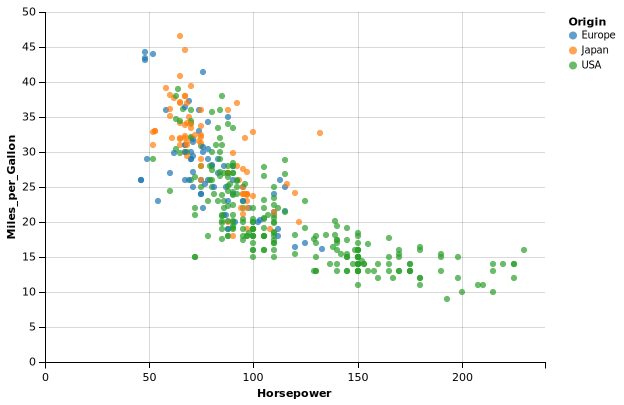
\includegraphics[width=12cm]{figures/vega.pdf}
% }
\begin{titlepage}
    \vspace*{\baselineskip}
    \vspace*{0.167\textheight} 
    Masterarbeit\\
    \vspace{\baselineskip}
    \begin{minipage}{15cm}
    {\huge Layout-Erkennung in digtalisierten Dokumenten mittels Neuronaler~Netzwerke\par}
    \end{minipage}
    
    \vspace{\baselineskip}
    von Jakob Schmolling\\
    \vfill
    Matrikelnummer:\\
    \vspace{\baselineskip}
    Datum: \today \\
    \vspace{\baselineskip}
    Fachbereich 4 Wirtschaftswissenschaften II\\
    Internationale Medieninformatik (M.A.)\\
    \vspace{\baselineskip}
    \begin{tabular}{@{\hspace{0em}}ll}
    Erstgutachter: & Prof. Dr. Klaus Jung\\
    Zweitgutachter: & Prof. Dr. Kai-Uwe Barthel\\
    \end{tabular}
\end{titlepage}
% \author{Jakob Schmolling}
% \title[]{
% \vfill
% \usebox{\titleimage}\\
% \noindent
% \huge{Layout-Erkennung in digtalisierten Dokumenten mittels Neuronaler Netzwerke}\\
% \noindent\Large{1.Korrektur}\\
% % \noindent\Large{Untertitel der Arbeit}\\
% % \noindent\Large{Untertitel der Arbeit}
% }


% \publisher[HTW Berlin]{HTW Berlin / \today}

\tableofcontents


\section*{Einleitung}
Diese Arbeit beschäftigt sich mit der Layout-Segmentierung von Digtalisierten Dokumenten mittels Neuronaler Netzwerke.

\cref{chap:documents} beschreibt die Motivation für die Dokumentensegmetierung und aktuelle Entwicklungen im
Bereich der Dokumenten-Digitaliserung.

\cref{chap:reproduktion} nähert sich dem aktuellen Forschungsstand mittels der Reproduktion von zwei Forschungsergebnissen.

\cref{chap:selfsupervised} erläuter die Methode des selbstüberwachten Lernen. Die Methode wird auf die reproduzierten Forschungen angewendet.

%-------------------------------------------------------------------------------
\chapter{Digitalisierte Dokumente}
\label{chap:documents}
% Warum scannt man Dokumente

% Was für Dokumente werden gescannt

% 
Schon in den 50er Jahren begann die Forschung im Bereich der Optischen Zeichenerkennung 
(engl. OCR)\autocite{doermann_evolution_2014}. OCR fand zuerst Anwendung in genau 
spezifizierten Problembereichen zum Beispiel die Erkennung von Druckbuchstaben einer Schreibmaschine. 
Je mehr Dokumente digitalisiert wurden, desto klarer wurde es das Dokumente mehr als 
eine Kette von Zeichen sind. 


Information wird in Dokumenten auch über die Position der Zeichen und Skalierung von Zeichen vermittelt.

Zum anderen bestehen Dokumente auch aus Inhalten die semantische Bedeutung haben, aber nicht als
Zeichenkette codiert werden können. 
Eine Randnotiz\marginnote{Der Bezug dieses Satzes zum Text wird durch die Position verdeutlicht} setzt sich durch Formatierung und Position vom restlichen Text ab. 


\section{Schritte in der Verarbeitung von Dokumentenbildern}
Die Dokumentensegmetierung ist ein Vorverarbeitungsschritt für weitere Schritte der Dokumentenverarbeitung.
Eine typische Aufgabe ist die Erkennung des Leseflüsses.

Im Bereich der Bibliotheswissenschaften besteht ein großes Interesse an Klassifizierung von
Buchseiten zur besseren Erschließung.
\cite{mcconnaughey_labeled_2017} klassifizieren Buchseiten anhand von textbasierten Features in 4 Kategorien. 
Flow

\section{Auswahl und Beschreibung der Datensätze}
\textcite[985\psqq]{doermann_datasets_2014} listen 5 Aspekte die bei der Erstellung von Datensätzen zu beachten sind:
Auswahl der Daten
Datenbeschaffung
Ground Truth Definition
Ground Trouth Annotation
Speicherformat
Struktur und Organisation

\section{DIVA-HisDB}
Der Datensatz DIVA-HisDB ist eine Sammlung von 150 Dokumentenseiten aus 3 mittelalterlichen Manuskripten \autocite{simistira_icdar2017_2017}.
\begin{itemize}
    \item CB55: \citefield{alighieri_cologny_1300}{title}
    \item CSG18: \citefield{ambrosius_st._985}{title}
    \item CSG863: \citefield{lucanus_st._1025}{title}
\end{itemize}
Die Manuskripte haben ein komplexes Layout und enthalten neben dem Haupttext auch Kommentare und Text-Dekorationen.
Die Manuskripte wurden mit einer Auflösung von 600 dpi gescannt und sind im  JPEG-Format gespeichert. 
Der Datensatz wurde manuell auf Pixelebene mit 4 Klassen annotiert (Hintergrund, Haupttext, Kommentar, Dekoration). Diese Ground-Truth-Annotationen sind im PAGE-XML-Format und als ``pixel-label'' PNG-Bilder gespeichert.


\begin{table*}
    \caption{Aufteilung der Seiten des DIVA-HisDB-Datenssets}

    \begin{tabular}{lccccc}
        {\bfseries Name} & {\bfseries Auflösung} & {\bfseries Training} & {\bfseries Validierung} & {\bfseries Test} & {\bfseries Test (ICDAR 2017)}\\
        \csvreader[head to column names]{tables/diva_hisdb_specs.csv}{}%
        {\name&	\width \(\times\)\height & \train	&\validate	&\test	&\comp\\}
    \end{tabular}
\end{table*}



%-------------------------------------------------------------------------------
\chapter{Reproduktion bisheriger Ergebnisse}
\label{chap:reproduktion}

\epigraph{What I cannot create, I do not understand}{--- Richarch Feyman}

\section{\textcite{chen_convolutional_2017}}
Superpixel segmentierung
Klassifizierung auf Superpixel statt Pixelebene.

\section{Bildverarbeitung mittels Neuronaler Netzwerke}
\section{CNN}
\section{SLIC Superpixel}
\cite{achanta_slic_2010}


\subsection{PyTorch}
% Genauer klären
PyTorch ist ein Framework zur automatischen Differenzierung von skaler Funktion \autocite{paszke_automatic_2017}.

\section{Dokumentensegmetierung mittels CNN}



\section{\textcite{xu_page_2017}}
\section{VGG}
\section{Deconvolution}

% \section{\textcite{wick_fully_2017}}
%-------------------------------------------------------------------------------
\chapter{Selbstüberwachtes Lernen}
\label{chap:selfsupervised}

Jigsaw
\cite{noroozi_unsupervised_2016}
% \begin{figure}
%     \includegraphics[]{figures/graphs/exp.pdf} 
%     \caption{Image}
%   \end{figure}
%-------------------------------------------------------------------------------
\chapter{Umsetzung}

\section{Evaluierung}

\sfigure{Beispiel aus dem DIBCO2013-Dateset}{figures/tasks/DIBCO2013-dataset.pdf}

\subsection{Metriken}
Die Evaluierung der Ergebnisse der Segmentierung erfolgt auf Pixelebene.
\cite{long_fully_2015} berechnet 4 Metriken.
Sei \(n_{ij}\) die Anzahl der Pixel der Klasse \(i\) die der Klasse \(j\) zugeordnet wurden.


\newcommand{\resulttable}[3]{
    \begin{tabular}{l|r|r|r|r|r}%
    \hline
        \csvreader[head to column names, filter equal={\dataset}{#2}]{#1}{}%
        {#3}
        \end{tabular}
}
\begin{table*}
    \resulttable{results/document_image_segmentation_results.csv}{CB55}{ \name & \pixelacc & \FgPA & \meanacc & \meanIU & \fwIU\\}
    \resulttable{results/document_image_segmentation_results.csv}{CSG18}{  \pixelacc & \FgPA & \meanacc & \meanIU & \fwIU\\}
    \resulttable{results/document_image_segmentation_results.csv}{CSG863}{  \pixelacc & \FgPA & \meanacc & \meanIU & \fwIU\\}
        
\end{table*}




\printbibliography[heading=bibintoc, title={Literaturverzeichnis}]\clearpage
% \printbibliography[heading=bibintoc, keyword={online}, title={Onlinequellen}]\clearpage
% \printbibliography[heading=bibintoc, keyword={image}, title={Bildquellen}]\clearpage

\pagebreak
\section*{Eidesstattliche Erklärung}
Hiermit versichere ich, dass ich die vorliegende Arbeit selbstständig verfasst und keine ande- ren als die angegebenen Hilfsmittel benutzt habe. Alle aus fremden Quellen im Wortlaut oder dem Sinn nach entnommenen Aussagen sind durch Angaben der Herkunft kenntlich gemacht.
Die Arbeit wurde bisher in gleicher oder ähnlicher Form keiner anderen Prüfungskommissi- on vorgelegt und auch nicht veröffentlicht.

\vspace{3cm}
\parbox{4cm}{\centering \hrule\strut \centering\footnotesize Ort, Datum} 
\hfill
\parbox{4cm}{\hrule\strut \centering\footnotesize Unterzeichner}

\end{document}